% MICCAI 2026 MSB EMERGE camera-ready, Springer LNCS template (llncs.cls).
% Based on the official "MICCAI2026-main conference paper template".
% Source paper: When Simple Wins (formerly final_report.tex, NeurIPS 2024 style).
\documentclass[runningheads]{llncs}
%
\usepackage[T1]{fontenc}
\usepackage{graphicx}
\usepackage{amsmath}
\usepackage{amsfonts}
\usepackage{booktabs}
\usepackage{nicefrac}
% hyperref loaded last; Springer eBook URL style:
\usepackage{color}
\usepackage{hyperref}
\renewcommand\UrlFont{\color{blue}\rmfamily}
\urlstyle{rm}
%
\begin{document}
%
\title{When Simple Wins: Lightweight CNN Encoders for Resource-Constrained Nucleus Segmentation}
\titlerunning{Lightweight CNN Encoders for Nucleus Segmentation}
%
\author{Danny Rollo}
\authorrunning{D. Rollo}
\institute{Northeastern University, Boston MA, USA \\
    \email{rollo.l@northeastern.edu}}
%
\maketitle
%
\begin{abstract}
For nucleus segmentation pipelines built without large annotated datasets or high-memory GPU infrastructure, a simple VGG U-Net encoder matches purpose-built transformer alternatives at a fraction of Swin-T's parameter count. We present a controlled comparison of VGG-style, ResNet-style, and Swin Transformer encoders within a shared U-Net framework, evaluated on PanNuke (${\sim}$5K training patches, 19 tissue types) and MoNuSeg (37 training whole-slide images). On PanNuke, VGG (Dice~0.854) matches ResNet (0.853) to within 0.002~Dice and outperforms pretrained Swin by 3.0~Dice points (0.824). On MoNuSeg, VGG (0.794) reaches published MedT-level performance---a transformer designed specifically for small medical datasets---while outperforming pretrained Swin by 3.6~Dice points (0.758). VGG is also the fastest and most memory-efficient of the learned models we test, making it Pareto-dominant over Swin-T at inference. In the deployment scenarios motivating this work---edge microscopy, veterinary and rare-disease research, and non-H\&E protocols where foundation-model pretraining misaligns---lightweight from-scratch architectures remain the practical choice, and a simple VGG encoder is the strongest of the three encoders we compare.

\keywords{Nucleus segmentation \and Histopathology \and U-Net \and Lightweight models \and Low-data.}
\end{abstract}

%% ============================================================================
\section{Introduction}
%% ============================================================================

Nucleus segmentation in histopathology images underlies a broad range of clinical and research workflows, from tumor microenvironment quantification to cell-cycle analysis. The dominant trend in computational pathology---scaling transformer-based foundation models to hundreds of millions of parameters pretrained on millions of whole-slide images~\cite{chen2024uni,vorontsov2024virchow}---addresses the challenge of limited labeled data but introduces new constraints on deployment.

Recent work has documented practical limits of this approach: foundation models are typically restricted to linear probing rather than full fine-tuning due to memory and stability constraints~\cite{tizhoosh2025why,campanella2025clinical}; their robustness to cross-site distribution shift has been questioned~\cite{dejong2025current}; and their H\&E-pretrained features transfer poorly to non-standard stains such as IHC~\cite{hua2024pathoduet}. For deployment scenarios such as edge-deployed microscopy in under-served settings~\cite{salido2025realtime} and veterinary or rare-disease research~\cite{xiao2025review}, where annotation budgets permit only tens of whole-slide images, lightweight from-scratch architectures remain the practical choice.

This raises a concrete design question: within the space of lightweight, from-scratch architectures, which encoder is best in the low-data regime? We answer it with a controlled ablation---a U-Net with a fixed decoder and shared encoder interface where the backbone is the only variable---comparing VGG, ResNet, and Swin encoders on PanNuke and the genuinely small-data MoNuSeg (37 images). A VGG encoder outperforms both ResNet and pretrained Swin on PanNuke and matches MedT (a transformer built for small medical datasets) while outperforming pretrained Swin on MoNuSeg.

While this resolution-vs-inductive-bias tradeoff is qualitatively well understood, we are not aware of prior work isolating encoder family as the sole variable across both a patch-scale and a genuinely small whole-slide-image benchmark, attributing the performance gap to architecture rather than to the recipe, data, and hyperparameter confounds that limit cross-paper comparisons.

\noindent\textbf{Contributions.} (1)~A controlled encoder-family ablation within a shared U-Net framework on PanNuke and MoNuSeg; (2)~evidence that a from-scratch VGG encoder matches MedT (a transformer purpose-built for small medical datasets) on MoNuSeg while beating pretrained Swin on both; (3)~inference-cost measurements showing VGG is Pareto-dominant over Swin-T in the lightweight regime.

\noindent\textbf{Code and dependencies.} We implement the U-Net, training loop, evaluation, and data loaders from scratch in PyTorch (\texttt{torchvision} for I/O and augmentation); the Swin encoder loads a \texttt{timm}~\cite{rw2019timm} backbone with pretrained ImageNet weights, PanNuke comes from HuggingFace \texttt{datasets}, MoNuSeg from the MICCAI 2018 challenge, and Otsu from \texttt{scikit-image}. Code, configurations, trained checkpoints, and exact dependency versions are available at \url{https://github.com/Bedrockdude10/BinaryCellSegmentation}.

%% ============================================================================
\section{Related Work}
%% ============================================================================

\noindent\textbf{U-Net}~\cite{ronneberger2015unet} introduced the symmetric encoder-decoder whose skip connections concatenate high-resolution encoder features into the decoder for precise localization; demonstrated on limited biomedical data, it remains the dominant medical segmentation backbone.

\noindent\textbf{Residual Networks}~\cite{he2016resnet} addressed degradation in deep networks via identity shortcuts; He et al.~\cite{he2015msra} separately proposed MSRA initialization for ReLU networks. Our ablation directly compares VGG- and ResNet-style encoders.

\noindent\textbf{Vision Transformers}~\cite{dosovitskiy2020vit} match CNNs on classification but require large-scale pretraining to compensate for the absence of convolutional inductive biases. The Swin Transformer~\cite{liu2021swin} adds shifted-window self-attention, producing hierarchical feature maps suited to dense prediction.

\noindent\textbf{Pathology Foundation Models.} UNI~\cite{chen2024uni} (307M parameters, 100K slides) and Virchow2~\cite{vorontsov2024virchow} (632M parameters, 1.5M slides) typify large-scale pathology pretraining. A clinical benchmark~\cite{campanella2025clinical} finds their gains concentrate on slide-level classification with more modest segmentation gains; Tizhoosh~\cite{tizhoosh2025why} documents heavy compute, poor robustness, and safety concerns; De~Jong et al.~\cite{dejong2025current} show they encode medical-center identity, limiting cross-site generalization; and PathoDuet~\cite{hua2024pathoduet} shows H\&E features need cross-stain training for IHC---motivating lightweight alternatives.

\noindent\textbf{MedT}~\cite{valanarasu2021medt}, our most directly relevant baseline, proposed gated axial-attention with a local-global (LoGo) training strategy for the small-medical-dataset regime. It reported Dice~0.7955 and IoU~0.6617 on the MoNuSeg test set (14 images), trained on 30 whole-slide images from the Kumar 2017 release~\cite{kumar2017monuseg}; we train on the 2018 expansion (37 images, $+$7).

\noindent\textbf{Instance-aware methods.} HoVer-Net~\cite{graham2019hovernet} predicts distance maps to separate overlapping nuclei beyond binary masks; HoVer-NeXt~\cite{hoverneXt2023} modernizes it with ConvNeXt-V2 backbones, and CellViT~\cite{cellvit2023} uses a histology-pretrained ViT. These run at higher complexity and larger data budgets than our target regime. We also exclude the widely used StarDist~\cite{schmidt2018stardist} and Cellpose~\cite{stringer2021cellpose}: their star-convex-polygon and flow-field targets, rather than binary masks, would introduce an annotation-format confound that conflicts with our single-variable design.

%% ============================================================================
\section{Methods}
%% ============================================================================

Our methodological contribution is a controlled ablation: we fix the decoder, training recipe, data pipeline, and evaluation protocol, varying only the encoder backbone across three representative families (VGG, ResNet, Swin), which isolates encoder choice as the single source of performance variation.

\subsection{Intuition}
\label{sec:intuition}

We expect CNNs to beat Swin in this low-data regime for three reasons (Otsu thresholding is a non-learned floor any reasonable model should clear). (i)~\emph{Skip-connection resolution}: nucleus boundaries are a few pixels wide, so the decoder needs high-resolution features; VGG preserves full $256\times256$ resolution at its first skip, whereas Swin's $4\times4$ tokenization downsamples $4\times$ immediately and bilinear upsampling cannot recover the detail. (ii)~\emph{Inductive bias vs.\ data scale}: self-attention needs more data than convolution to learn translation-equivariance and local-structure priors---unlikely at ${\sim}$5K PanNuke patches or 37 MoNuSeg images, even with ImageNet pretraining (an H\&E domain mismatch). (iii)~\emph{Input scale}: on $256\times256$ patches a stacked-$3\times3$ VGG receptive field already covers most of the input by stage~4, limiting global attention's value. Section~\ref{sec:experiments} tests these, including whether residual connections or loss choice matter at four stages.

\subsection{Architecture}
\label{sec:architecture}

Our pipeline uses a U-Net with a fixed decoder and a shared encoder interface: each encoder's \texttt{forward(x)} returns four feature maps at progressively lower resolutions and exposes per-stage channel counts, which the decoder reads dynamically---so swapping backbones requires only configuration changes.

\subsubsection{Decoder.}
The decoder is a bottleneck block followed by four upsampling stages, each a transposed convolution, concatenation with the matching encoder skip connection, and a two-layer conv block (batch normalization~\cite{ioffe2015batchnorm} and ReLU); a final $1\times1$ convolution produces single-channel logits. Batch normalization follows every convolution in all encoders.

\subsubsection{VGG Encoder.}
The VGG encoder follows the design principles of~\cite{simonyan2014vgg}: four stages of stacked $3\times3$ convolutions with batch normalization and ReLU, with max-pooling between stages for spatial downsampling. Channel widths double at each stage: $64 \to 128 \to 256 \to 512$. Features are stored \emph{before} pooling to preserve full spatial resolution for skip connections, producing outputs at $256^2$, $128^2$, $64^2$, and $32^2$ for $256\times256$ inputs. Total parameters: ${\sim}34$M.

\subsubsection{ResNet Encoder.}
The ResNet encoder replaces plain convolutional blocks with residual blocks~\cite{he2016resnet}. A lightweight $3\times3$ stem (stride 1) replaces the standard ResNet stem to match VGG's spatial dimensions. Downsampling in stages 2--4 uses stride-2 convolution in the first block of each stage, with $1\times1$ projection shortcuts. Channel widths match VGG. Total parameters: ${\sim}37.5$M.

\subsubsection{Swin Transformer Encoder.}
The Swin encoder wraps a Swin-T backbone~\cite{liu2021swin} via \texttt{timm}, with channels $96 \to 192 \to 384 \to 768$. Its $4\times4$ tokenization natively yields features at $\nicefrac{H}{4}$, $\nicefrac{H}{8}$, $\nicefrac{H}{16}$, $\nicefrac{H}{32}$---lower resolution than the CNN encoders at every stage---which we bilinearly upsample to $256^2$, $128^2$, $64^2$, $32^2$. We evaluate randomly initialized and ImageNet-pretrained variants. Total parameters: ${\sim}87$M.

\subsection{Loss Functions}

We compare two losses on sigmoid-activated logits: per-pixel Binary Cross-Entropy (BCE) and region-based Dice loss, which directly optimizes the Dice coefficient and handles class imbalance:
\begin{align*}
\mathcal{L}_{\text{BCE}} = -\tfrac{1}{N}\textstyle\sum_i \big[y_i \log\hat{y}_i + (1-y_i)\log(1-\hat{y}_i)\big],
\qquad
\mathcal{L}_{\text{Dice}} = 1 - \frac{2\sum_i \hat{y}_i y_i + \epsilon}{\sum_i \hat{y}_i + \sum_i y_i + \epsilon}.
\end{align*}

\subsection{Classical Baseline}

Otsu thresholding~\cite{otsu1979threshold} is the non-learned floor: each test image is converted to grayscale and thresholded at the intensity maximizing between-class variance, classifying darker pixels as nuclei (nuclei appear darker than background in H\&E). It has zero learnable parameters and requires no training.

\subsection{Datasets}
\label{sec:datasets}

\noindent\textbf{Data use declaration.} Both datasets are publicly available and released under the CC BY-NC-SA 4.0 license; they comprise de-identified, previously published images, so no additional ethics approval was required for this work.

\noindent\textbf{PanNuke}~\cite{gamper2019pannuke,gamper2020pannuke_ext} provides 7,904 $256\times256$ patches across 19 tissue types with 189,744 nuclei in 5 categories, pre-split into three folds. We train on fold1, validate on fold2, and evaluate on fold3; binary masks collapse all cell-type labels to foreground. Augmentation is random flips and $90^\circ$ rotations with ImageNet normalization.

\noindent\textbf{MoNuSeg}~\cite{kumar2017monuseg} provides 37 training whole-slide images ($1000\times1000$, H\&E, XML polygon annotations over 7 organs) and 14 test images whose lung and brain organs are absent from training, testing generalization to unseen tissue. We use the 2018 expansion.\footnote{The public challenge description lists 30 training images (the original 2017 release); the training set distributed for the 2018 challenge, which we use, contains 37. MedT reports the 30-image count.} Images are reflection-padded to $1024\times1024$ and tiled into 16 non-overlapping $256\times256$ patches; validation is carved at the image level (20\%, seed 42) so no slide spans both splits. Test images are tiled identically, with per-image Dice averaged over 16 patches.

\subsection{Training Details}
\label{sec:training_details}

All models train with SGD (momentum 0.9, weight decay $10^{-4}$, batch size 8), with early stopping on validation Dice and consistent augmentation and ImageNet normalization. CNN encoders use learning rate $0.01$ with step decay ($\gamma=0.1$ at epoch 30); pretrained Swin uses $10^{-4}$ with cosine annealing. On \textbf{PanNuke}, patience is 15 (CNNs converge in 48--50 epochs); on \textbf{MoNuSeg}, patience is 20 with a 100-epoch cap (CNN) or 150 (Swin).

%% ============================================================================
\section{Experiments and Results}
\label{sec:experiments}
%% ============================================================================

% TODO(camera-ready): Table 3 still holds the Apple M3 inference numbers. If you
% switch it to the V100 measurement in runs/_bench/, say so here as well.
\noindent\textbf{Testbed.} Accuracy results are averaged over 5 training seeds, all
run on a single NVIDIA Tesla~V100-SXM2-32GB in fp32; inference cost
(Table~\ref{tab:inference_cost}) is measured on an Apple~M3 with the PyTorch MPS
backend (unified memory, no discrete GPU). Training uses batch size 8 and the recipe of Section~\ref{sec:training_details}, using the shared framework of Section~\ref{sec:architecture} with only the encoder swapped. Data pipeline, augmentation, optimizer, and decoder are fixed to isolate backbone choice. Metrics are Dice and IoU on the held-out splits (PanNuke fold3; MoNuSeg 14-image test set).

\noindent\textbf{Research questions.} We address five questions: encoder family (Q1) and the effect of ImageNet pretraining (Q2) on PanNuke; whether the CNN advantage holds in the low-data regime and a VGG encoder reaches MedT's published performance (Q3) on MoNuSeg; whether residual shortcuts or Dice loss help at four encoder stages (Q4); and whether inference cost matches the lightweight-deployment framing (Q5).

\subsection{PanNuke Results}

Table~\ref{tab:pannuke_results} summarizes results on PanNuke fold3; all learned models substantially exceed the classical Otsu baseline. VGG and ResNet produce nearly identical results (0.854 vs.\ 0.853 Dice): the
paired difference is 0.002~Dice (95\% CI $[0.001, 0.002]$), reproducible across
seeds but an order of magnitude below the ${\sim}0.005$ Dice we treat as
practically meaningful, so we do not rank them.
% TODO(camera-ready): the two sentences below are the ONE place the new data
% changes the argument, not just the numbers. Measured at n=5: from-scratch Swin
% 0.825 +- 0.001 vs pretrained 0.824 +- 0.001, paired difference +0.001 Dice
% (95% CI [+0.001,+0.002]) in favour of FROM-SCRATCH. ImageNet pretraining
% therefore yields no benefit here, and the published "+0.212 lift" came from a
% single from-scratch run that diverged (its per-epoch val Dice oscillated
% 0.278/0.531/0.003/0.023/0.585...). Note this STRENGTHENS the "not a matter of
% weights" reading: if ImageNet weights change nothing measurable, the residual
% ~0.03 gap to VGG cannot be about those weights. Rewrite in your own voice;
% do not write "pretraining significantly hurts" -- 0.001 Dice is immaterial.
Addressing Q1--Q2: Swin underperforms both CNN encoders by roughly 3~Dice points,
with or without ImageNet pretraining. This 0.030 Dice gap (paired, 95\% CI
$[0.029, 0.031]$) is an order of magnitude larger than the BCE-vs-Dice variation
for a fixed encoder (0.002 Dice), indicating a genuine architectural effect
rather than seed noise.

\begin{table}[t]
\centering
\caption{Test results on PanNuke fold3, mean $\pm$ standard deviation over 5
training seeds ($n{=}5$; the Otsu baseline is deterministic). Epochs is the
early-stopping epoch. Best result in \textbf{bold}.}
\label{tab:pannuke_results}
\begin{tabular}{@{}llcccr@{}}
\toprule
\textbf{Encoder} & \textbf{Loss} & \textbf{Dice} $\uparrow$ & \textbf{IoU} $\uparrow$ & \textbf{Epochs} & \textbf{Params} \\
\midrule
Otsu (classical) & --- & 0.482 & 0.349 & --- & 0 \\
\midrule
Swin-T (scratch) & BCE & 0.825 $\pm$ 0.001 & 0.703 $\pm$ 0.002 & 69.0 $\pm$ 9.4 & 86.8M \\
Swin-T (pretrained) & BCE & 0.824 $\pm$ 0.001 & 0.701 $\pm$ 0.001 & 96.2 $\pm$ 5.0 & 86.8M \\
ResNet & BCE & 0.853 $\pm$ 0.000 & 0.743 $\pm$ 0.001 & 49.8 $\pm$ 3.8 & 37.5M \\
VGG & Dice & \textbf{0.856} $\pm$ \textbf{0.001} & \textbf{0.748} $\pm$ \textbf{0.001} & 84.8 $\pm$ 17.5 & 34.0M \\
VGG & BCE & 0.854 $\pm$ 0.000 & 0.746 $\pm$ 0.000 & 51.8 $\pm$ 2.6 & 34.0M \\
\bottomrule
\end{tabular}
\end{table}

\subsection{MoNuSeg Results}
\label{sec:monuseg_results}

Table~\ref{tab:monuseg_results} shows MoNuSeg test results (14 images, per-image averaged Dice), answering Q3. VGG reaches Dice~0.794~$\pm$~0.011, close to MedT's published 0.796 but
not comparable to it on equal terms, and outperforms pretrained Swin by 3.6~points (0.758~$\pm$~0.007;
paired difference 0.036, 95\% CI $[0.021, 0.052]$). The MedT comparison is not strictly controlled (different training-set size and input protocol; see Limitations), so we read it only as VGG \emph{reaching} MedT-level Dice. That caveat is confined to this cross-paper anchor: VGG, ResNet, and Swin share the identical 37-image set and protocol, so our controlled VGG-over-Swin result is unaffected;
the gap is comparable at both data scales.

\begin{table}[t]
\centering
\caption{Test results on MoNuSeg (14 test images). Dice computed per image, averaged over the test set. MedT results are published figures (30 training images, $512\times512$ input); ours use 37 training images, $256\times256$ patches, reported as mean $\pm$
standard deviation over 5 training seeds ($n{=}5$). Best result in \textbf{bold}.}
\label{tab:monuseg_results}
\begin{tabular}{@{}lccc@{}}
\toprule
\textbf{Model} & \textbf{Dice} $\uparrow$ & \textbf{IoU} $\uparrow$ & \textbf{Params} \\
\midrule
MedT~\cite{valanarasu2021medt} (published, 30 imgs) & 0.796 & 0.662 & 1.4M \\
Swin-T (pretrained, ours, 37 imgs) & 0.758 $\pm$ 0.007 & 0.613 $\pm$ 0.008 & 86.8M \\
VGG (ours, 37 imgs) & \textbf{0.794} $\pm$ \textbf{0.011} & \textbf{0.660} $\pm$ \textbf{0.015} & 34.0M \\
\bottomrule
\end{tabular}
\end{table}

\begin{figure}[t]
\centering
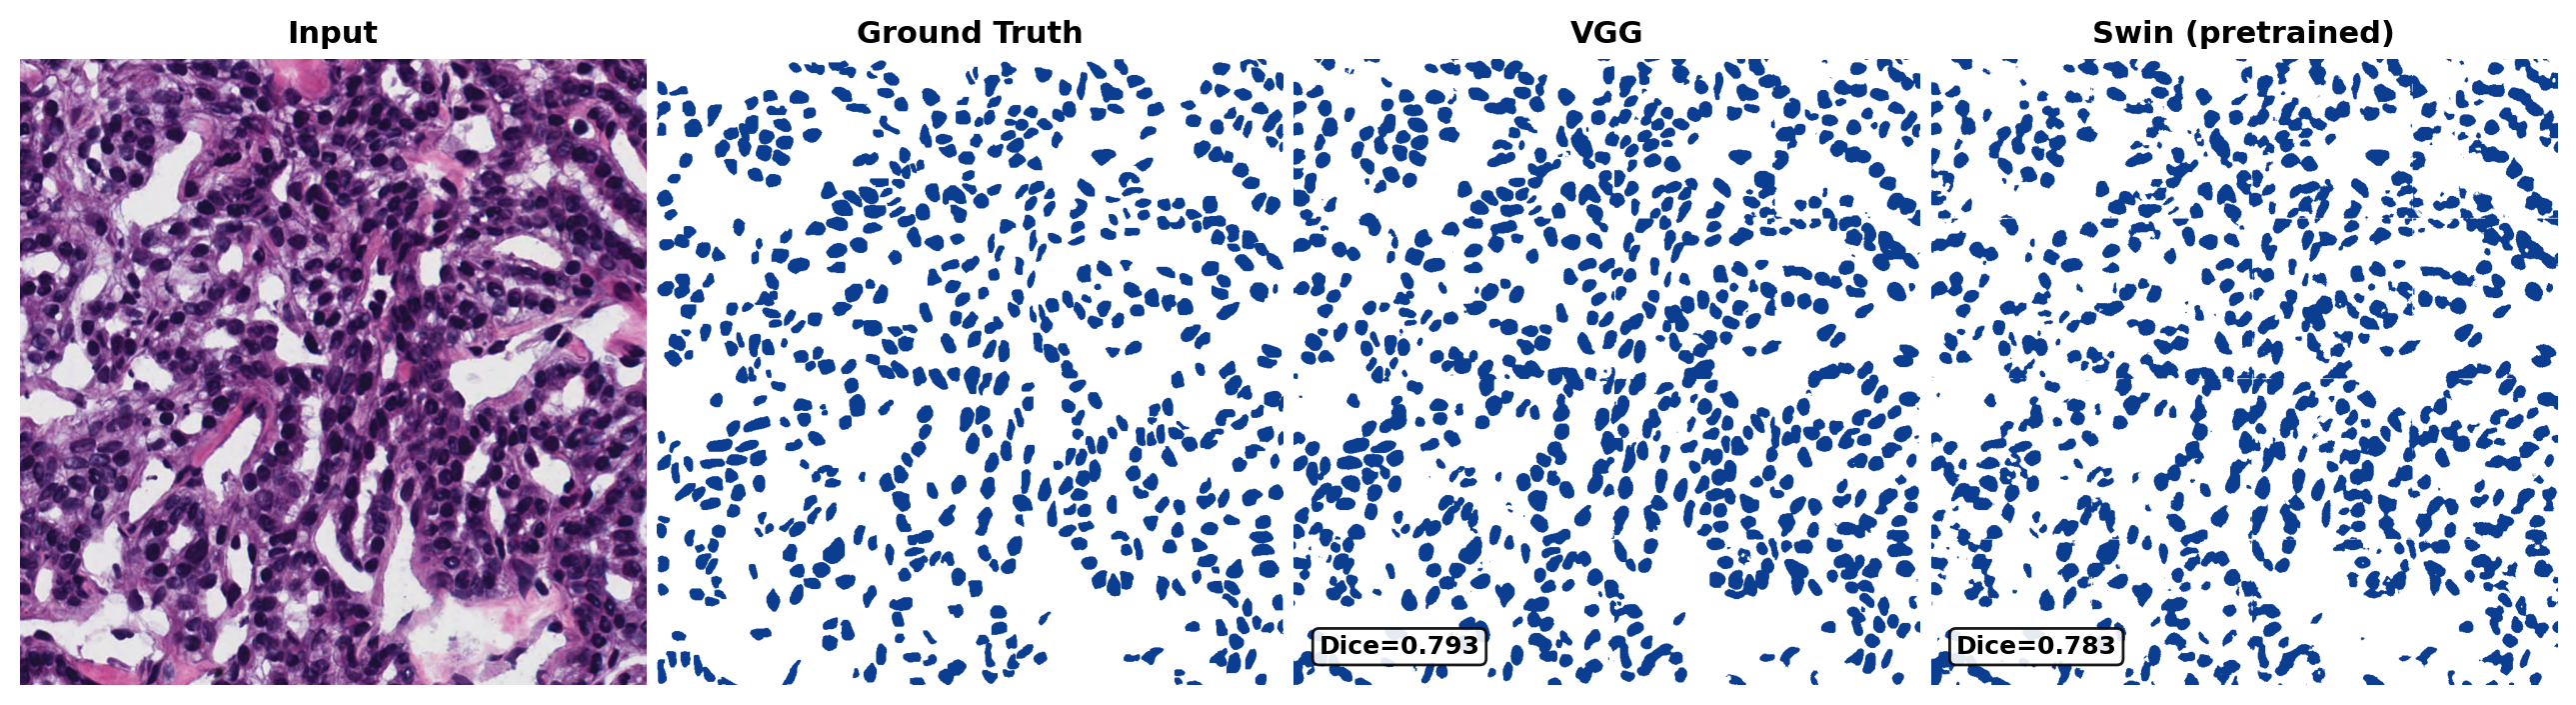
\includegraphics[width=\textwidth]{figures/monuseg_comparison_row1_seed42_solid.png}
\caption{Qualitative comparison on a representative dense MoNuSeg test region. Left to right: input H\&E patch, ground-truth nucleus overlay (green), VGG prediction, and pretrained Swin prediction (per-image Dice annotated in each prediction cell). VGG delineates nuclear boundaries more tightly; Swin produces smoother masks with less precise boundaries.}
% TODO(authorial A7): this caption claim is now weaker on this slide. The
% regenerated figure (seed 42) annotates VGG 0.793 vs Swin 0.783 -- a 0.010 gap
% against Table 2's 0.036 mean, so the region under-represents the effect.
% Options: (a) keep and soften the wording; (b) switch to
% figures/monuseg_comparison_row1_seed42_errormap.png, which shows FP/FN directly
% and supports the boundary claim better, but needs the column description
% rewritten (columns become per-pixel agreement, not predictions);
% (c) pick a more representative slide -- but say so in the caption if you do,
% since choosing the region that best shows the effect is otherwise
% cherry-picking. The three candidate renders are all in figures/.
\label{fig:monuseg_qualitative}
\end{figure}

\subsection{Residual Connections and Loss (Q4)}

VGG and ResNet produce nearly identical PanNuke results (0.854 vs.\ 0.853 Dice):
residual connections matter mainly in \emph{deep} networks~\cite{he2016resnet}, and
at four stages neither suffers gradient degradation, so shortcuts add no benefit
worth having---we recommend VGG for its simpler implementation. BCE and Dice loss
are likewise near-identical (0.854 vs.\ 0.856 Dice; 0.746 vs.\ 0.748 IoU). Both
differences are reproducible across seeds yet below 0.005~Dice, so we report them
as measurable but immaterial rather than as rankings. With moderate foreground
density BCE is not hurt by class imbalance, and Dice helps only with very sparse
foreground.

\subsection{Inference Cost}
\label{sec:inference_cost}

Table~\ref{tab:inference_cost} reports inference cost on our testbed (mean forward-pass latency over 100 iterations on a single $256\times256$ input after a 10-iteration warmup; peak memory via \texttt{torch.mps.current\_allocated\_memory}), answering Q5. These support the lightweight-deployment framing rather than serving as optimized benchmarks (eager-mode PyTorch, no fusion or quantization).

\begin{table}[t]
\centering
\caption{Single-image inference cost at $256\times256$ on Apple~M3 / MPS, batch size~1. Latency is the mean over 100 forward passes after warmup. VGG is the fastest and most memory-efficient learned model.}
\label{tab:inference_cost}
\begin{tabular}{@{}lrrr@{}}
\toprule
\textbf{Model} & \textbf{Params} & \textbf{Latency (ms)} & \textbf{Peak Memory (MB)} \\
\midrule
VGG U-Net & 34.0M & 25.2 & 130.5 \\
ResNet U-Net & 37.5M & 34.2 & 144.0 \\
Swin-T U-Net (pretrained) & 86.8M & 46.6 & 333.6 \\
\bottomrule
\end{tabular}
\end{table}

Swin uses roughly $2.6\times$ the memory and $1.8\times$ the latency of VGG for no accuracy gain; pathology foundation models in the 300M--1B range~\cite{chen2024uni,vorontsov2024virchow} need about an order of magnitude more inference memory and are typically deployed via linear probing on cached embeddings~\cite{tizhoosh2025why,campanella2025clinical}. A VGG U-Net fits comfortably on a consumer laptop GPU; even Swin-T already costs meaningfully more.

\subsection{Qualitative Analysis}

Qualitatively (Fig.~\ref{fig:monuseg_qualitative}), Swin's $4\times4$ tokenization and bilinear upsampling yield smoother, less precise boundaries than the CNN encoders; all models struggle with dense overlapping clusters that binary masks cannot resolve into instances.

%% ============================================================================
\section{Discussion}
%% ============================================================================

\noindent\textbf{Implications for resource-constrained deployment.} Foundation models are memory-hungry and, depending on hardware, may be unusable; they are typically limited to linear probing rather than full fine-tuning~\cite{tizhoosh2025why}. A VGG U-Net (${\sim}34$M parameters) instead trains overnight on a single 8GB consumer GPU with no external data---directly actionable for the edge-microscopy, veterinary, and non-H\&E settings~\cite{xiao2025review,neal2025artificial} that motivate this work.

% TODO(camera-ready): REWRITE. At n=5 ImageNet pretraining closes NOTHING: from-
% scratch 0.825 +- 0.001 vs pretrained 0.824 +- 0.001. The "+0.212 Dice" figure
% came from one diverging from-scratch run. The skip-connection mechanism you
% attribute the gap to is unaffected and is now supported more directly, since
% the weights demonstrably make no difference. Gap to VGG is 0.030, not 0.049.
\noindent\textbf{The role of pretraining.} Pretraining does not fail on Swin---it closes most of the Otsu-to-CNN gap ($+$0.212 Dice)---but cannot close the final 0.049 to VGG, which we attribute to the skip-connection resolution bottleneck (Section~\ref{sec:intuition}): a property of the architecture, not the weights. This predicts that even domain-matched pretraining (e.g., UNI~\cite{chen2024uni}) would narrow but not close the gap---a falsifiable target for future work.

\subsection{Limitations}

% TODO(camera-ready): REWRITE the variance sentence -- it is now false and it is
% the reviewers' central objection. Replacement facts: every configuration in
% Tables 1 and 2 was re-run over 5 training seeds on one GPU model with one fixed
% split; mean +- SD reported; comparisons paired per seed with 95% CIs; all 11
% paired CIs on test Dice exclude zero. Remaining honest limitations: this
% measures TRAINING-SEED variance only, on a single fixed split, so it says
% nothing about split or dataset variance; n=5 does not support Wilcoxon
% (its two-sided floor is p=0.0625 at n=5); and pretrained Swin reached its
% 100-epoch cap in 2 of 5 seeds -- a 150-epoch cosine schedule lifts it to
% 0.830 +- 0.001, still 0.025 below VGG.
Several limitations bound these conclusions. All results are single runs without variance estimates, though the order-of-magnitude gap between architectural and loss effects in our PanNuke results is indirect evidence of stability. We study only binary segmentation, not instance separation of touching nuclei (flagged in our qualitative analysis); the MedT comparison is uncontrolled in training-set size (37 vs.\ 30) and protocol ($256\times256$ tiles vs.\ a single $512\times512$ pass); and all data are H\&E, leaving the non-H\&E stains (IHC, fluorescence) that most motivate this work untested.

%% ============================================================================
\section{Conclusion}
%% ============================================================================

We compared CNN and transformer encoders for nucleus segmentation under real-world resource constraints. In a shared U-Net on PanNuke and MoNuSeg, a from-scratch VGG encoder (34M parameters) outperforms pretrained Swin on both and reaches published MedT-level performance on MoNuSeg (0.794 vs.\ 0.796 Dice, a rough equivalence given protocol differences)---a margin consistent across both data scales and matching our hypothesized skip-connection-resolution mechanism. For pipelines with tens of annotated images and single-GPU infrastructure, a VGG U-Net encoder is thus the strongest of the three encoders we compare; transformers need large-scale pretraining or far more data to match it.

\noindent\textbf{Future work.} Promising directions: a resolution-matched Swin variant, or a CNN with equivalently reduced skip resolution, to separate tokenization from encoder family; a domain-matched pretraining source in place of ImageNet; the data scale at which pretrained Swin matches VGG; hybrid CNN-transformer encoders; and memory-matched comparison with foundation models (UNI, Virchow2).

%
% ---- Bibliography (LNCS style, alphabetical by first-author surname) ----
%
\begin{thebibliography}{99}

\bibitem{hoverneXt2023}
Baumann, E., Dislich, B., Rumberger, J.L., Nagtegaal, I.D., Mart\'inez, M.R., Zlobec, I.: HoVer-NeXt: a fast nuclei segmentation and classification pipeline for next generation histopathology. In: Medical Imaging with Deep Learning (MIDL). PMLR, vol.~250, pp. 61--86 (2024)

\bibitem{salido2025realtime}
Bueno, G., S\'anchez-Vargas, L., D\'iaz-Maroto, A., Ruiz-Santaquiteria, J., Blanco, M., Salido, J., Crist\'obal, G.: Real-time edge computing vs.\ GPU-accelerated pipelines for low-cost microscopy applications. Electronics \textbf{14}(5), 930 (2025)

\bibitem{campanella2025clinical}
Campanella, G., Chen, S., et al.: A clinical benchmark of public self-supervised pathology foundation models. Nat. Commun. \textbf{16}, 3640 (2025)

\bibitem{chen2024uni}
Chen, R.J., Ding, T., Lu, M.Y., Williamson, D.F.K., et al.: Towards a general-purpose foundation model for computational pathology. Nat. Med. \textbf{30}(3), 850--862 (2024)

\bibitem{dejong2025current}
de Jong, E.D., et al.: Current pathology foundation models are unrobust to medical center differences. arXiv:2501.18055 (2025)

\bibitem{dosovitskiy2020vit}
Dosovitskiy, A., Beyer, L., Kolesnikov, A., Weissenborn, D., Zhai, X., Unterthiner, T., Dehghani, M., Minderer, M., Heigold, G., Gelly, S., Uszkoreit, J., Houlsby, N.: An image is worth 16x16 words: transformers for image recognition at scale. In: International Conference on Learning Representations (ICLR) (2021)

\bibitem{gamper2019pannuke}
Gamper, J., Koohbanani, N.A., Benet, K., Khuram, S.A., Rajpoot, N.: PanNuke: an open pan-cancer histology dataset for nuclei instance segmentation and classification. In: European Congress on Digital Pathology (ECDP), pp. 11--19 (2019)

\bibitem{gamper2020pannuke_ext}
Gamper, J., Koohbanani, N.A., Graham, S., Jahanifar, M., Khurram, S.A., Azam, A., Hewitt, K., Rajpoot, N.: PanNuke dataset extension, insights and baselines. arXiv:2003.10778 (2020)

\bibitem{graham2019hovernet}
Graham, S., Vu, Q.D., Raza, S.E.A., Azam, A., Tsang, Y.W., Kwak, J.T., Rajpoot, N.: HoVer-Net: simultaneous segmentation and classification of nuclei in multi-tissue histology images. Med. Image Anal. \textbf{58}, 101563 (2019)

\bibitem{he2015msra}
He, K., Zhang, X., Ren, S., Sun, J.: Delving deep into rectifiers: surpassing human-level performance on ImageNet classification. In: IEEE International Conference on Computer Vision (ICCV), pp. 1026--1034 (2015)

\bibitem{he2016resnet}
He, K., Zhang, X., Ren, S., Sun, J.: Deep residual learning for image recognition. In: IEEE Conference on Computer Vision and Pattern Recognition (CVPR), pp. 770--778 (2016)

\bibitem{cellvit2023}
H\"orst, F., Rempe, M., Heine, L., et al.: CellViT: vision transformers for precise cell segmentation and classification. Med. Image Anal. \textbf{94}, 103143 (2024)

\bibitem{hua2024pathoduet}
Hua, S., Yan, F., Shen, T., Ma, L., Zhang, X.: PathoDuet: foundation models for pathological slide analysis of H\&E and IHC stains. arXiv:2312.09894 (2024)

\bibitem{ioffe2015batchnorm}
Ioffe, S., Szegedy, C.: Batch normalization: accelerating deep network training by reducing internal covariate shift. In: International Conference on Machine Learning (ICML), pp. 448--456 (2015)

\bibitem{kumar2017monuseg}
Kumar, N., Verma, R., Sharma, S., Bhargava, S., Vahadane, A., Sethi, A.: A dataset and a technique for generalized nuclear segmentation for computational pathology. IEEE Trans. Med. Imaging \textbf{36}(7), 1550--1560 (2017)

\bibitem{liu2021swin}
Liu, Z., Lin, Y., Cao, Y., Hu, H., Wei, Y., Zhang, Z., Lin, S., Guo, B.: Swin Transformer: hierarchical vision transformer using shifted windows. In: IEEE International Conference on Computer Vision (ICCV), pp. 10012--10022 (2021)

\bibitem{neal2025artificial}
Neal, S.V., et al.: Artificial intelligence in veterinary clinical pathology---an introduction and review. Vet. Clin. Pathol. (2025)

\bibitem{otsu1979threshold}
Otsu, N.: A threshold selection method from gray-level histograms. IEEE Trans. Syst. Man Cybern. \textbf{9}(1), 62--66 (1979)

\bibitem{ronneberger2015unet}
Ronneberger, O., Fischer, P., Brox, T.: U-Net: convolutional networks for biomedical image segmentation. In: Medical Image Computing and Computer-Assisted Intervention (MICCAI), pp. 234--241 (2015)

\bibitem{schmidt2018stardist}
Schmidt, U., Weigert, M., Broaddus, C., Myers, G.: Cell detection with star-convex polygons. In: Medical Image Computing and Computer-Assisted Intervention (MICCAI), pp. 265--273 (2018)

\bibitem{simonyan2014vgg}
Simonyan, K., Zisserman, A.: Very deep convolutional networks for large-scale image recognition. arXiv:1409.1556 (2014)

\bibitem{stringer2021cellpose}
Stringer, C., Wang, T., Michaelos, M., Pachitariu, M.: Cellpose: a generalist algorithm for cellular segmentation. Nat. Methods \textbf{18}, 100--106 (2021)

\bibitem{tizhoosh2025why}
Tizhoosh, H.R.: Why foundation models in pathology are failing. arXiv:2510.23807 (2025)

\bibitem{valanarasu2021medt}
Valanarasu, J.M.J., Oza, P., Hacihaliloglu, I., Patel, V.M.: Medical Transformer: gated axial-attention for medical image segmentation. In: Medical Image Computing and Computer-Assisted Intervention (MICCAI), pp. 36--46 (2021)

\bibitem{vorontsov2024virchow}
Vorontsov, E., Bozkurt, A., Casson, A., et al.: A foundation model for clinical-grade computational pathology and rare cancers detection. Nat. Med. \textbf{30}(10), 2924--2935 (2024)

\bibitem{rw2019timm}
Wightman, R.: PyTorch Image Models. \url{https://github.com/huggingface/pytorch-image-models} (2019)

\bibitem{xiao2025review}
Xiao, S., Dhand, N.K., Wang, Z., Hu, K., Thomson, P.C., House, J.K., Khatkar, M.S.: Review of applications of deep learning in veterinary diagnostics and animal health. Front. Vet. Sci. \textbf{12}, 1511522 (2025)

\end{thebibliography}
\end{document}
